\newpage
\section{Revisão da Teoria}

\subsection{Modulação PSK}

Na modulação por chaveamento de fase, os bits de informação são codificados na fase do sinal transmitido, durante um intervalo de símbolo $T_s$. Para a modulação BPSK (Binary Phase Shift Keying), somente 1 bit é transmitido por símbolo, assim, $T_s = T_b$, sendo $T_b$ o período de bit.

A expressão geral para representação de um conjunto de sinais com modulação de fase da portadora no domínio tempo é:

\begin{equation}
s_k(t) = A_c \cdot p_T(t) \cdot cos(2 \pi f_c t + D_p \cdot m(t)).
\end{equation}

Onde:

\begin{itemize}
	\item $A_c$ é a amplitude do sinal;
	
	\item $p_T(t)$ é a formatação do pulso transmitido;
	
	\item $D_p$ é a constante do modulador de fase;
	
	\item e $m(t)$ é a informação binária a ser transmitida.
\end{itemize}

A Figura \ref{fig:bpsk} ilustra um exemplo da modulação BPSK.


	\begin{figure}[H]
		\centering
		\caption{Exemplo de mensagem modulada com chaveamento por deslocamento de fase.}
		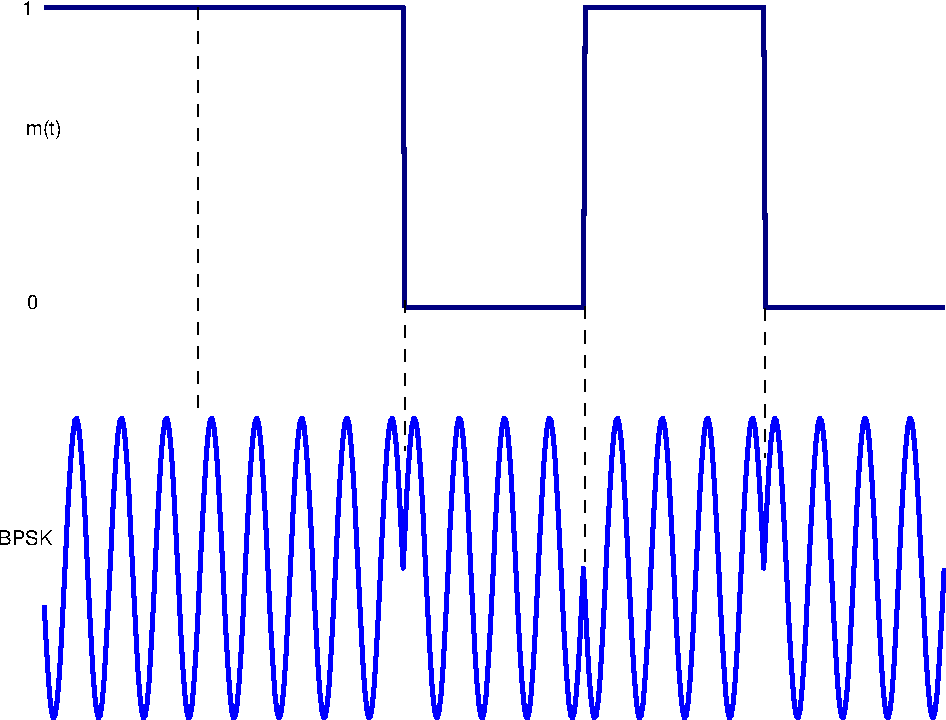
\includegraphics[scale=0.6]{bpsk}
		
		\small Fonte: Abrão, T., Modulação e Sistemas de Comunicação Digital, 2017 [2].
		\label{fig:bpsk}
	\end{figure}

Para este tipo de modulação deve-se usar a detecção síncrona, já que esta tem como base o conhecimento preciso a respeito da fase da onda portadora recebida, bem como da sua frequência. Esta técnica de modulação devido ao fato mencionado, envolve circuitos de recepção (demodulação) mais sofisticados; em compensação oferece melhor desempenho que as técnicas ASK e FSK. A Figura \ref{fig:txrx} apresenta um modelo do transmissor e receptor BPSK.

	\begin{figure}[H]
		\centering
		\caption{Transmissor e receptor BPSK.}
		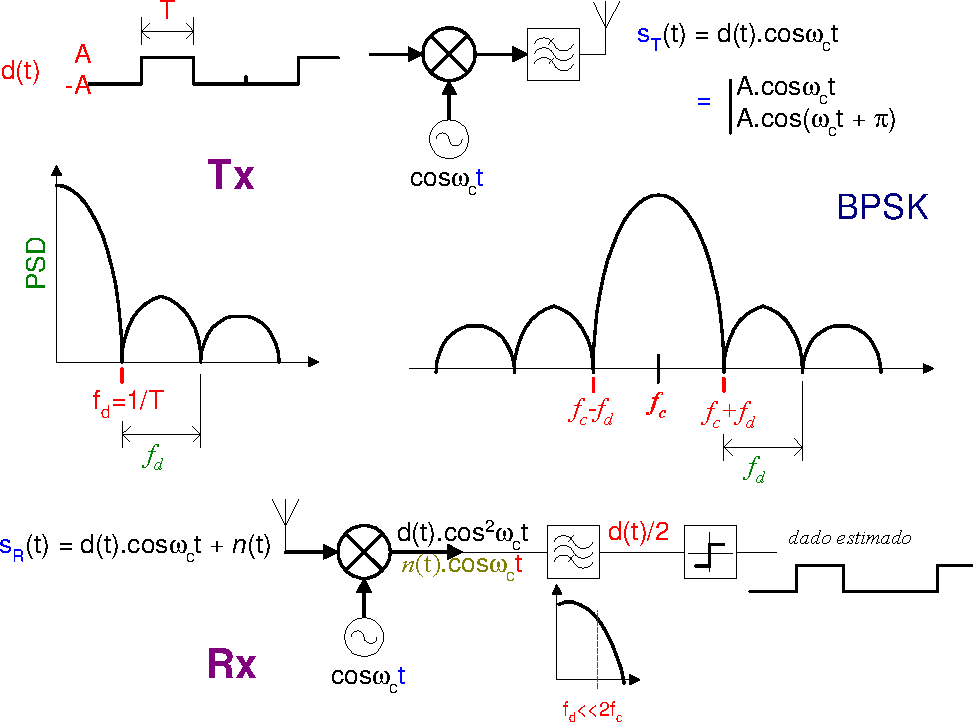
\includegraphics[scale=0.6]{txrx}
		
		\small Fonte: Abrão, T., Modulação e Sistemas de Comunicação Digital, 2017 [2].
		\label{fig:txrx}
	\end{figure}

Para este trabalho, a modulação será obtida adicionando uma componente em quadratura, representada por $Q$ e que pode ser revertida em fase, em uma portadora constante representada na Figura \ref{fig:fasor} pelo fasor $C$,  de modo a fornecer um sinal resultante de fase $\pm \phi$.

	\begin{figure}[H]
		\centering
		\caption{Diagrama de fasor do chaveamento por deslocamento de fase PSK.}
		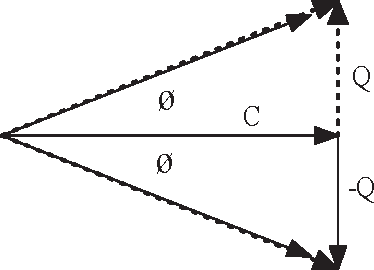
\includegraphics[scale=1]{fasor}
		
		\small Fonte: Jacob, J. L., Roteiro de laboratório, 2017 [1].
		\label{fig:fasor}
	\end{figure}
	
\subsection{Demodulação PSK}

Para a demodulação do sinal BPSK, o receptor deve reconstruir um sinal como referência de fase, equivalente ao fasor C na Figura \ref{fig:fasor}, para que a fase do sinal recebido possa ser comparada. 

O sinal de referência de fase pode ser gerado com um circuito PLL (\textit{Phase Locked Loop}) desde que o formato dos dado seja tal que os períodos dos sinais 0 e 1 ocorram em um pequeno intervalo. O PLL deve er uma ação lenta o suficiente para manter o oscilador no meio das duas fases dos sinais. A codificação bi-fase poder ser utilizada para viabilizar a geração da fase de referência com o circuito PLL.

De forma simplificada, a fase de referência pode ser extraída da fase média do sinal recebido, estabelecendo, através de um PLL, um sinal em quadratura com este.

A demodulação pode então ser realizada através da modulação deste último sinal com o sinal recebido.